% !TEX TS-program = pdflatex
% !TEX encoding = UTF-8 Unicode

\documentclass[11pt]{article} % use larger type; default would be 10pt

\usepackage[utf8]{inputenc} % set input encoding (not needed with XeLaTeX)

%%% PAGE DIMENSIONS
\usepackage{geometry}
\geometry{letterpaper}

\usepackage{graphicx} % support the \includegraphics command and options

% \usepackage[parfill]{parskip} % Activate to begin paragraphs with an empty line rather than an indent

%%% PACKAGES
\usepackage{booktabs} % for much better looking tables
\usepackage{tabularx}
\usepackage{caption}
\usepackage{array} % for better arrays (eg matrices) in maths
\usepackage{paralist} % very flexible & customisable lists (eg. enumerate/itemize, etc.)
\usepackage{verbatim} 
\usepackage{subfig} 
\usepackage{siunitx} % for easier number formatting
\usepackage{units} % added back in


%%%  LINE NUMBERS
\usepackage{lineno}
\linenumbers

%%% HEADERS & FOOTERS
\usepackage{fancyhdr} % This should be set AFTER setting up the page geometry
\pagestyle{fancy} % options: empty , plain , fancy
\renewcommand{\headrulewidth}{0pt} % customise the layout...
\lhead{}\chead{}\rhead{}
\lfoot{}\cfoot{\thepage}\rfoot{}

%%% SECTION TITLE APPEARANCE
\usepackage{sectsty}
%\allsectionsfont{\sffamily\mdseries\upshape} % (See the fntguide.pdf for font help)
% (This matches ConTeXt defaults)

%%% ToC (table of contents) APPEARANCE
\usepackage[nottoc,notlof,notlot]{tocbibind} % Put the bibliography in the ToC
\usepackage[titles,subfigure]{tocloft} % Alter the style of the Table of Contents
\renewcommand{\cftsecfont}{\rmfamily\mdseries\upshape}
\renewcommand{\cftsecpagefont}{\rmfamily\mdseries\upshape} % No bold!

\title{IceCube Instrumentation and Online Systems}
\author{The IceCube Collaboration}
\date{}

\begin{document}
\maketitle

%!TEX TS-program = pdflatex
%!TEX root = i3det-top.tex
%!TEX encoding = UTF-8 Unicode

\section{Introduction}
\label{sec:intro}

\subsection{IceCube Science}
\textsl{(1 page)}

\subsection{A Functional Description of the IceCube Instrument}

\textit{testtest}

In order to observe astrophysical neutrinos, the primary science goal of the experiment, IceCube exploits the fact that charged particles moving through
the ice at super-luminal speed emit Cherenkov photons. An enormous detection volume is required since the cross-sections of neutrinos are small for producing secondary charged particles in interactions with ordinary matter. The glacial ice cap at the South Pole is about \SI{3}{\kilo\meter} thick and therefore predestined as operation site since it is not only offering aplenty interaction material but also a medium with unmatched high quality. 
Cherenkov light is produced in cascades of neutrino-induced muons penetrating the deep, other high-energy particles as well as generated by by cosmic-ray muons that result from cosmic-ray interactions in the atmosphere above Antarctica. 
Due to a Cherenkov photon yield of $\mathcal{O}(\num{E5})$ visible photons per \SI{}{\giga\electronvolt} of shower energy, the long optical attenuation length in South Pole ice and large-area photomultipliers (PMTs) it is possible to instrument cubic kilometers of ice with a rather wide spacing of detectors.  
The basic detection unit in IceCube in order to capture the Cherenkov light is the digital optical module or \textit{DOM} which is covered in great detail in Sec.~\ref{sec:dom}. Encapsulated in a \SI{1/2}{''} thick glass pressure sphere to withstand the extreme pressure in the deep ice, the main components of a DOM are a \SI{10}{''} PMT, embedded high-voltage generation, a flasher calibration board, and a mainboard containing the analog and digital processing circuitry for PMT pulses. 
%The transmission of the digital data is controlled by an FPGA and embedded processor hosted on the mainboard. 
The digitized data is fed to a central computing facility at the surface via a unique cable system, see Sec.~\ref{sec:cable}. 
Aspects of detector deployment and ice drilling are covered in Sec.~\ref{sec:drill-deploy}.
An overview of the data flow as well as its readout, processing and filtering are subjects of Sec.~\ref{sec:online} where we also cover the data handling, monitoring and operational performance of the observatory.
The IceCube instrument consists of three sub-detectors -- IceCube, DeepCore and IceTop -- using the same instrumentation design of embedded digital optical modules and associated surface readout. A schematic layout of the array is shown in Fig.~\ref{fig:array} 

\begin{figure}[!h]
 \centering
 \includegraphics[width=0.8\textwidth]{graphics/intro/ArrayWSeasonsLabels_crop.pdf}
 \caption{The IceCube Neutrino Observatory with its sub-array DeepCore and the air shower array IceTop.}
 \label{fig:array}
\end{figure}


\subsubsection{IceCube}
In order to detect the Cherenkov photons emitted by charged particles traversing the ice, \num{5160} DOMs are deployed between \SI{1450}{\meter} and \SI{2450}
{\meter} below the glacial surface on \num{86} vertical strings each holding \num{60} DOMs deployed along a copper cable. The main \textit{deep-ice} array consists of \num{78} strings with a vertical separation of the DOMs on each string of \SI{17}{\meter}. These strings are deployed on a hexagonal grid with \SI{125}{\meter} horizontal spacing and spanning a volume of one cubic kilometer of ice. 
\textit{Talk about energy range covered by this instrumentation and primary science goal}

\subsubsection{DeepCore}

The remaining subset of in-ice DOMs is deployed in the deep ice below a depth of \SI{1750}{\meter} forming a denser instrumented volume. This sub-array, the DeepCore \cite{ICECUBE:DC} consists of eight specialized and closely spaced strings of sensors located around the central IceCube string.
Its inter-string spacings of \SI{75}{\meter} and inter-DOM spacings of \SI{7}{\meter} are optimized for the detection of atmospheric neutrinos with energies typically in the range from \SI{100}{\giga\electronvolt} to \SI{400}{\tera\electronvolt} \cite{ICECUBE:AtmNu}.

\subsubsection{IceTop}

IceTop \cite{ICECUBE:IceTop} consists of \num{81} clear ice-filled  Cherenkov tanks that are arranged in pairs on the same, approximately \SI{125}{\meter}, triangular grid as the vertical cables that carry the deep sensors of IceCube. The two tanks at each surface station are separated from each other by \SI{10}{\meter}. Each tank contains two standard IceCube DOMs. Air showers initiated in the atmosphere by cosmic rays are typically spread over a number of stations. The light generated in the tanks by the shower particles (electrons, photons, muons and hadrons) is a measure of the energy deposit of these particles in the tanks.




\clearpage

%auto-ignore

% additional definitions
\newcommand{\degC}[1]{$\unit[#1]{^\circ{C}}$}
% definition to produce a "less than or similar to" symbol
\def\lsim{\mathrel{\rlap{\raise 0.2ex\hbox{$\,<\,$}}{\lower 0.9ex\hbox{$\,\sim\,$}}}}
% definition to produce a "greater than or similar to" symbol
\def\gsim{\mathrel{\rlap{\raise 0.2ex\hbox{$\,>\,$}}{\lower 0.9ex\hbox{$\,\sim\,$}}}}


\section{\label{sec:dom}The Digital Optical Module}

\subsection{\label{sec:dom_functional}A Functional Description of the DOM}

The DOM is the fundamental light sensor and data acquisition unit for IceCube.
It consists of a spherical glass housing 
containing a downward-facing \SI{10}{''} diameter PMT~\cite{ICECUBE:PMT}
and associated circuit boards that allow near-autonomous operation (figure~\ref{fig:domcomponents}).
Data acquisition, control, calibration, communication, and low-voltage power conversion 
are integrated in one annular circuit board (Main Board) that fits around the neck of the PMT~\cite{ICECUBE:DAQ}. 
Separate circuit boards generate PMT high voltage, interface to the PMT pins,
delay PMT signals, and generate calibration light flashes that can reach other DOMs.
Key requirements for the DOM include
the precise recording of a wide variety of PMT pulse widths and amplitudes
with nanosecond time resolution, robustness in 
a challenging deployment environment, and long-term reliability.

%============================================================

\begin{figure}[!h]
  \captionsetup[subfigure]{labelformat=empty}
  \centering
  \subfloat[]{\includegraphics[width=0.5\textwidth]{graphics/dom/functional/domfig1a-DOM3DModel.pdf}}
  \subfloat[]{\includegraphics[width=0.5\textwidth]{graphics/dom/functional/domfig1b-DOMBlockDiagram.pdf}}
  \caption{Components of the DOM, showing mechanical layout (left) and functional connections (right).}
  \label{fig:domcomponents}
\end{figure}

%============================================================


The PMT detects signals from particles interacting in the ice, typically ranging over
energies from \unit[10]GeV to \unit[10]PeV and distances up to \unit[500]m
away.  At a gain of $10^7$ (section~\ref{sec:hv}), corresponding PMT waveforms can have amplitudes from \unit[1]mV up
to and beyond the linearity limit of the PMT (\unit[$\sim2$]V) and widths
from \unit[12]ns up to around \unit[1500]ns.  In order to accommodate such a variety
of signals, the DOM includes multiple digitizers with overlapping dynamic
range and different sampling speeds
(section~\ref{sec:mainboard}).  Each DOM independently
detects individual photons, starting a recording of
the PMT waveform that also includes photons arriving up to
\unit[6.4]{$\mu$s} later (a ``hit'').  The hit time is saved along with the
waveform shape, allowing the determination of the times of arriving photons
relative to this reference.  The DOM accumulates such hit
data for a period of about \unit[1]s before sending the data up as a block.
However, if data readout is interrupted, the DOM can store
$\mathcal{O}(\SI{10}{\second})$ of data before overflowing local memory
(16MB of SDRAM), depending on hit rate.  Separately, the PMT hit rate is recorded by
the DOM in \unit[1.6384]ms intervals, as a collective increase of all rates
could signify detection of many low energy neutrinos in case of a Galactic
supernova event (section~\ref{sect:SNDAQ}) \cite{IC3:supernova}.

DOMs transmit their data to computers in the ICL
over a twisted wire pair that also provides power (section~\ref{sec:cable}).
Wire pairs are bundled to form the vertical in-ice cables and the horizontal surface
cables.  Each wire pair is shared between two DOMs, with data transfers
initiated by a surface computer.  Separately, dedicated local coincidence
(LC) wiring to neighbor DOMs above and below allows quick recognition of neighboring
coincident hits, where
nearest or next-to-nearest neighbors are hit within a common time
window. The time window is configurable and is set to $\pm1~\mu\mathrm{s}$
for both in-ice and IceTop DOMs. The signals are forwarded from one DOM to the next
through the dedicated wiring.  The span of the forwarding is
software-configurable and is currently set to two for in-ice DOMs,
i.e. a DOM signals its neighbor and next-to-nearest neighbor DOMs in
both up and down directions along the string. The local coincidence
connections for IceTop, which allow coincidences between the two tanks in a
station, are described in ref.~\cite{ICECUBE:IceTop}. Local coincidence
hits (``HLC'' hits) often have complex PMT waveforms
indicating multiple photons detected in each DOM and are therefore saved
in full detail; otherwise, the DOM saves abbreviated information appropriate
to single photon detection (section~\ref{sect:online:payloads}).

The DOM is capable of interpreting commands from the surface that specify
tasks for configuration, data taking and transmission, monitoring or
self-calibration.  Self-calibration functions establish PMT and amplifier
gains as well as sampling speed (section~\ref{sec:domcal}).  The RAPCal
system (section~\ref{sect:dom:rapcal}) is implemented for tracking each
local DOM clock's offset from universal time, allowing PMT pulses that were
independently recorded in many DOMs to be built into events by surface
computers.

\subsection{\label{sec:dom_components}Components}

\subsubsection{\label{sec:sphere}Glass Sphere and Harness}

The glass sphere housing has an outer diameter of \SI{13}{''} and thickness
of \SI{0.5}{''}.
The spheres protect the inside electronics and PMT against long-term applied pressure of 
\unit[250]bar (\unit[2.6]km-equivalent water depth)
as well as temporary overpressure up to \unit[690]bar during the refreezing of melted ice in the drill hole.
The housings were produced by Benthos (Falmouth, Massachusetts), based on a design for deep-sea
environments but using borosilicate glass from Kopp Glass
with very low potassium and other radioactive trace elements that would contribute to the dark noise
count rate (section~\ref{sect:darknoise}).  
Optical transmission was measured in representative glass samples as 93\% at \unit[400]nm,
decreasing to 50\% at \unit[340]nm and 10\% at \unit[315]nm (normal
incidence). Fresnel reflection is not included in the quoted
transmission, since the effect of Fresnel reflection is small in ice,
where the refractive index is better matched to the glass.

All spheres were tested up to \unit[690]bar hydrostatic pressure by the manufacturer.
Each was delivered as two hemispheres that mate precisely at the equator
and were sealed during assembly (section~\ref{sec:dom_prodtest}).  The DOM
is held by an aluminum waistband with rubber gaskets against 
the glass above and below the equator seam. 
Figure~\ref{fig:domcable} shows how the DOM is attached to the main in-ice cable via a harness
of steel rope and chain that carries the weight load around the DOM.
The main cable bends around the DOM, and the DOM axis stays vertically aligned with the string.

%============================================================
\begin{figure}
\vspace{3pt}
\centering
\begin{tabular}{c@{\hspace{0.5in}}c}
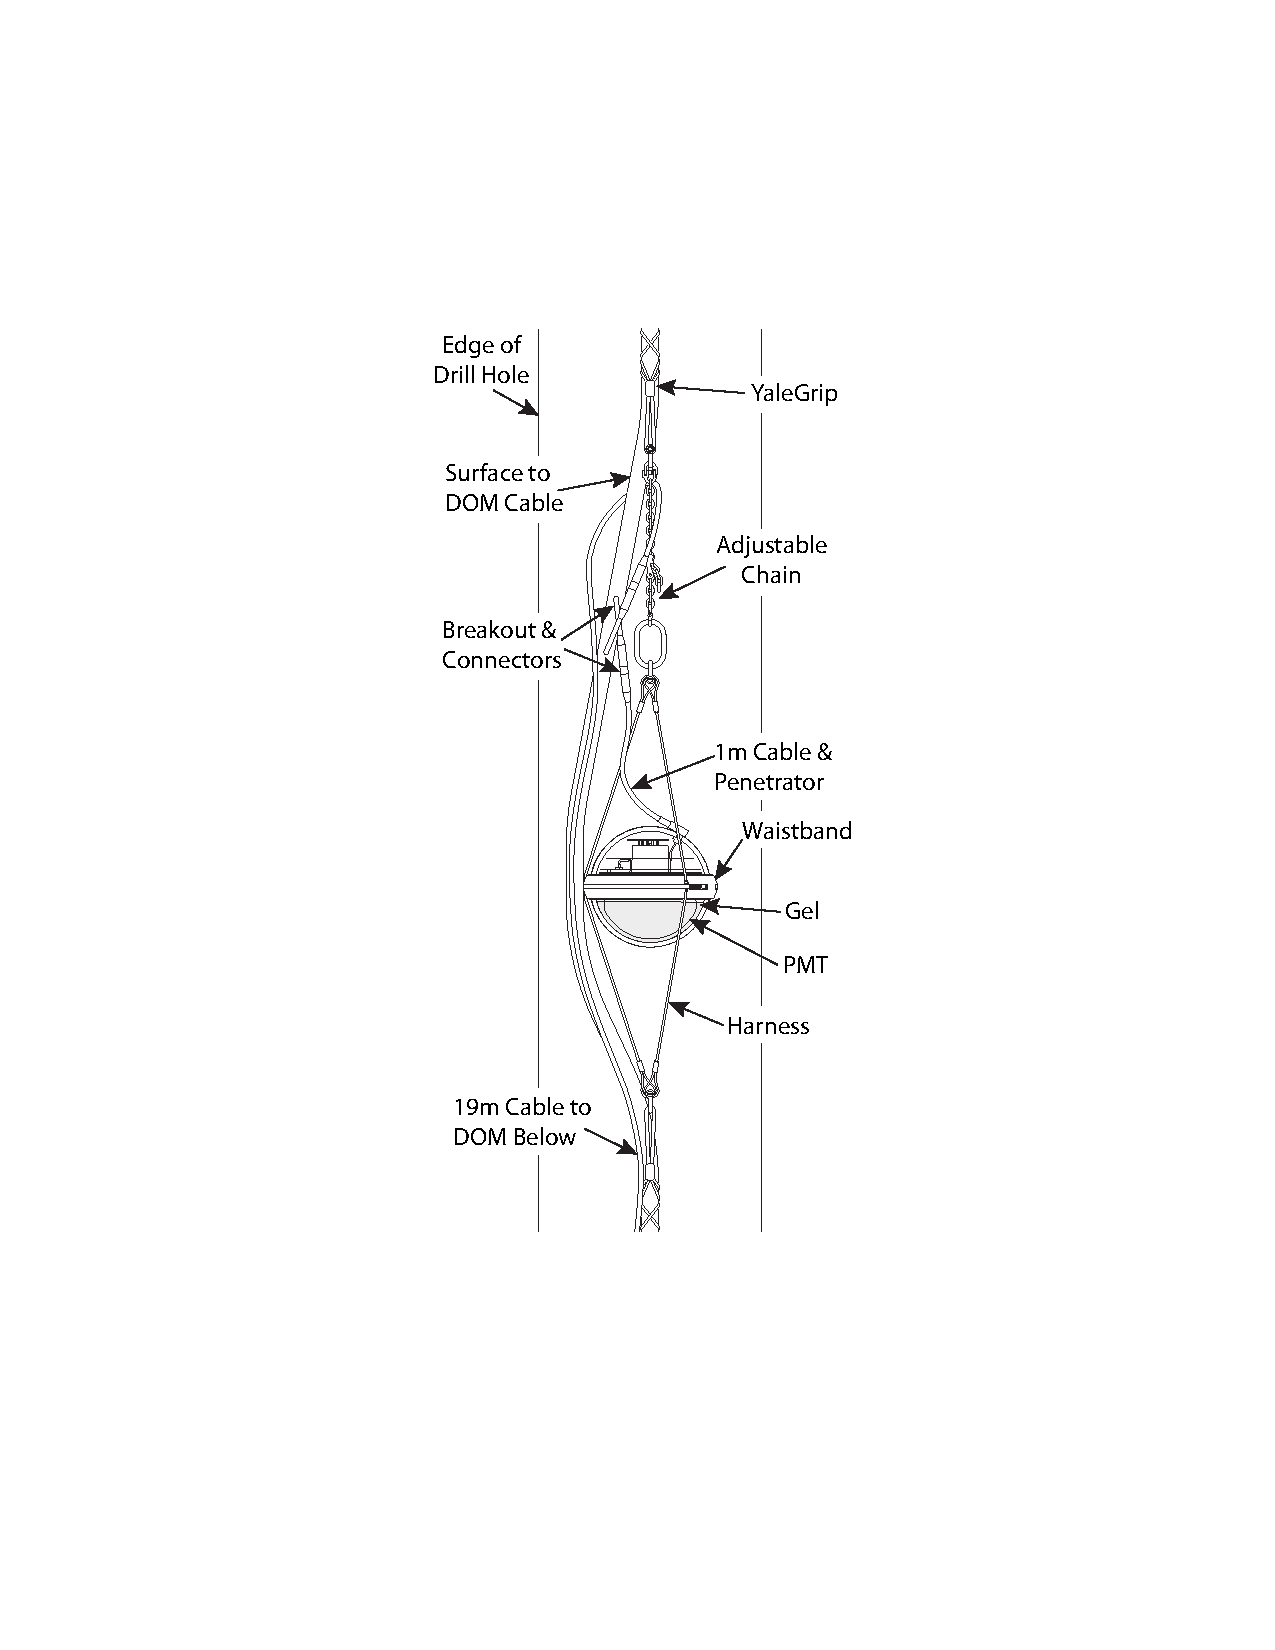
\includegraphics[width=0.4\textwidth,clip=true]{graphics/dom/functional/domfig2a-CableAssembly.pdf} & \
\includegraphics[width=0.45\textwidth,clip=true]{graphics/dom/functional/domfig2b-CableConnections.pdf} \\
\end{tabular}
\caption{
(Left) DOM as deployed on main in-ice cable, showing cable breakout to the penetrator
assembly and the mechanical support system.  (Right) Schematic of cable connections for a set
of four DOMs serviced by two wire pairs from the surface that carry power and
communications.  The ``T'' labels indicate where electrical termination (\unit[140]$\Omega$) is
installed in one of two DOMs that share such a wire pair.  Other wire pairs are used for
bidirectional signaling between neighboring DOMs, in order to check for in-time coincident
detections.
}
\label{fig:domcable}
\end{figure}
%============================================================

\subsubsection{\label{sec:penetrator}Cable Penetrator, Cable and Connector}

A penetrator assembly brings three wire pairs out through a \unit[16.3]mm hole in
the DOM glass sphere.  The wires are routed inside a customized cable, shown in figure~\ref{fig:domcable},
and terminate at a pressure-tight, waterproof connector that mates with a similar connector
that continues each pair into the main cable.  One wire pair carries power and a
bidirectional digital communications stream, connecting ultimately
with a computer in the
IceCube Laboratory building (section~\ref{sec:cable}).
The other wires lead to neighboring DOMs directly above and below,
carrying LC digital pulses that signify time-correlated hits in nearby DOMs (section~\ref{sec:mainboard}).

DOMs were produced in two versions, in which the communications wire pair was either electrically
terminated (\unit[140]$\Omega$) or unterminated inside the DOM.  The
terminated DOM is deployed \unit[17]m below the unterminated one (\unit[7]m
or \unit[10]m in DeepCore strings) and therefore includes a correspondingly 
long penetrator assembly cable (figure~\ref{fig:domcable}).

The entire penetrator assembly was designed and produced by SEACON Brantner \& Associates (El Cajon,
California).  The part that seals against the DOM glass is a
hollow steel bolt that is secured inside the DOM by a nut and spring
washer and compresses a fluorosilicone O-ring against the outside surface.
The steel part includes additional sealing around the wires that pass
through it.  Outside the DOM, a plastic shell is molded around the steel
and onto the cable jacket.  External mechanical features like the
penetrator are subject to large stresses during deployment and the
refreezing process; a right-angle bend outside the DOM was included for
robustness, based on previous experience deploying AMANDA modules.

\subsubsection{\label{sec:pmt}PMT, Gel and Magnetic Shield}

DOMs use the \SI{10}{''}-diameter Hamamatsu R7081-02 PMT, 
or the corresponding high-quantum-efficiency (HQE) version, Hamamatsu R7081-02MOD, for DeepCore strings.
The PMT properties have been measured and described in ref.~\cite{ICECUBE:PMT}.
The PMT is specified by Hamamatsu for the wavelength range
\unit[300]nm--\unit[650]nm, with peak quantum efficiency around 25\% (34\%
for HQE) near \unit[390]nm.  It features a box-and-line dynode chain with 10 stages,
with in-ice DOMs (both standard and HQE) operated at a gain of $10^7$ (section~\ref{sec:domcal}).

The PMT bulb faces downwards in the bottom glass hemisphere, secured in high-strength 
silicone gel to a depth sufficient to surround the photocathode area.  
The gel provides both good optical coupling and mechanical support for the
whole assembly of PMT and circuit boards. The gel thickness between PMT
envelope and glass sphere is approximately \unit[1]cm.   
Originally the gel was supplied from General Electric as RTV6136-D1,
and later as a similar formulation from Quantum Silicones (Virginia, USA).  
It is optically clear with transmission of 97\% at \unit[400]nm, 91\% at \unit[340]nm, and 65\% at \unit[300]nm
(normal incidence).  The refractive index is 1.41, yielding less than 0.1\% reflection as light
passes from the sphere glass into the gel and then into the PMT envelope.
The characteristics of the cured gel are specified to remain stable in the
temperature range $-70^\circ$C to $45^\circ$C.  Visual inspection of
non-deployed DOMs reveals no indication of crazing after more than 10
years, and studies of the long-term optical efficiency of deployed DOMs
reveal no measurable aging effects (section~\ref{sec:optical_stability}).  

To reduce effects of the ambient South Pole magnetic field (\unit[550]mG, $17^\circ$
from vertical) on the PMT collection efficiency, a mu-metal cage surrounds the PMT bulb up to
the neck.  It was constructed as a wire mesh with typical wire spacing \unit[66]mm and
wire diameter \unit[1]mm, blocking about 4\% of the incident light,
and delivered by ITEP Moscow.
Without such a shield, this PMT exhibits 5-10\% lower
collection efficiency, poorer single photoelectron resolution, and gain variations of 20\% depending on 
azimuthal orientation, for a South Pole magnetic field strength and orientation~\cite{calvo}.
With the shield in place, the interior magnetic field is 2.8 times
smaller than the external field, pointing mostly along the axis and therefore reducing efficiency by
less than 2\% for this type of PMT.

Other interior DOM components are held in place by attachment to the PMT, mostly via screws into
a molded plastic collar glued around the PMT neck.  The PMT Base Board is
soldered directly to the PMT pins.

\subsubsection{\label{sec:hv}High Voltage Supply and Divider}

The PMT high voltage subsystem consists of a resistive 
voltage divider circuit (PMT Base Board) directly
solder-mounted on the PMT and a separate High Voltage Control Board. 
The High Voltage Control Board includes a DAC and ADC for setting and reading out the PMT high voltage,
connected to the Main Board with a digital interface, as well as the high
voltage generator itself.

The high voltage generator is a custom encapsulated module (\#9730A) designed by
EMCO High Voltage (California).  The maximum high voltage is
\unit[2047]volts, specified for up to $30\,{\rm \upmu A}$ current.  The
voltage setting, in steps of 0.5V, is controlled by the DAC
output, and the actual voltage is monitored via a high-impedance divider and the ADC.  The output ripple
is less than \unit[1]mV, and stability is better than \unit[1]V RMS.  Power
consumption of the high voltage supply is less than \unit[300]mW at full
load. 

The generator output is carried to the PMT Base Board \cite{ICECUBE:PMT} via a high voltage
coaxial cable.  The voltage divider, designed for low power consumption,
presents a total resistive load of \unit[130]M$\Omega$. 
The PMT is operated with cathode at ground potential, so the anode signal output is AC-coupled using 
a 1:1 bifilar-wound toroid transformer mounted on the Base Board; this
toroid was modified once during DOM production in order to reduce
distortion of high-amplitude signals (section~\ref{sec:waveformcal}).
The transformer secondary is then wired to the Main Board analog input with a coaxial cable.
The single photoelectron (SPE) output waveform has been described in ref.~\cite{ICECUBE:PMT}.  
With a \unit[100]$\Omega$ load connected to the transformer, and operating
at standard PMT gain of $10^7$, the SPE 
peak voltage before front-end amplification is approximately \unit[8]mV
with a FWHM of \unit[7--8]ns.  Several effects combine to increase
the FWHM of digitized SPE waveforms to $\sim$\unit[13]ns (peak $\sim$\unit[5]mV).

\subsubsection{\label{sec:mainboard}Main Board and Delay Board}

The Main Board, designed at Lawrence Berkeley National Laboratory,
has been described in detail in \cite{ICECUBE:DAQ}.   
Essentially an embedded single-board data-acquisition computer, the Main
Board interfaces to other boards as shown in figure~\ref{fig:domcomponents} and
provides many key functions of the DOM, including:

\begin{enumerate}
\item{Control of all the devices inside the DOM, including the high voltage power supply for the PMT, 
the flasher board, and various sensors (pressure, temperature, power supply voltage monitor). 
Also supplies necessary DC power to the subsystems.}
\item{Digitization of the PMT waveforms, using a custom integrated circuit (ATWD: Analog
  Transient Waveform Digitizer~\cite{ICECUBE:DAQ}) and a continuously sampling fast ADC (fADC).}
\item{Providing computational functions, including PMT gain calibration, compressing 
digitized waveforms, temporarily storing the data, and creating time-stamped data packets.}
\item{Communicating with the data acquisition (DAQ) system on the surface.}
\item{Exchanging timing pulses with the surface DAQ to calibrate the internal DOM clock. }
\item{Exchanging LC pulses with the adjacent DOMs.}
\item{Uniquely identifying each DOM by providing a Main Board ID generated from a 
component device identifier.}
\item{Providing an onboard adjustable low-intensity optical source
    for direct calibration of PMT gain and timing, and hosting a
    daughter board with an adjustable high-intensity optical source for inter-module calibration.}
\end{enumerate}

The data flow starting from the PMT is shown in figure~\ref{fig:domdataflow}.
PMT waveforms are amplified and compared to a discriminator threshold.  Two
discriminators are available, the SPE discriminator that is used for in-ice DOMs
and typically set to a voltage threshold corresponding to \unit[0.25]PE,
and an MPE discriminator used for the larger-amplitude signals in IceTop.
A discriminator crossing begins a "launch" of the high speed waveform
capture and digitization. Each DOM is equipped with two ATWD chips,
and each chip is provided with three different amplifier
gains with nominal values of 16, 2, and 0.25 in order to completely cover the 
dynamic range of the PMT output (up to 150~mA, or 7.5V, when saturated).  A
fourth ATWD channel on each chip is used for calibration inputs and is not normally read out.
The ATWD chips are configured to sample the input voltage at \unit[300]Msps
and operate by analog storage of waveform samples in switched capacitor arrays of depth 128,
followed by a 10-bit digitization \cite{atwd}.  In order to record the waveform starting from before the discriminator
threshold crossing, the signal is first routed through the Delay Board.  Here a total delay of about
\unit[75]ns is accomplished by an approximately \unit[10]m-long, \unit[0.25]mm-wide
serpentine copper trace embedded in the dielectric and sandwiched between
ground planes.  The highest-gain channel is used
for most pulses, and lower-gain recordings are also retained as needed when pulses reach 75\% of the range 
of a higher-gain channel, in order to avoid any loss of information due to
digital saturation.  The mean amplifier gains of all deployed DOMs for high-,
medium-, and low-gain channels are $15.7\pm0.6$, $1.79\pm0.06$, and $0.21\pm0.01$ respectively.

\begin{figure}[h]
 \centering
 \includegraphics[width=0.9\textwidth]{graphics/dom/functional/domfig3-DOMDataFlow.pdf}
 \caption{Data flow diagram for recording and processing of PMT waveforms in the DOM to form 
 "Hit Records" that are sent to the surface DAQ computers.  As shown by dashes, full waveform data are only included
 when neighbor DOMs report time-coincident signals above the SPE discriminator threshold.  Additionally,
 data from low gain channels are omitted for waveforms that are within range of higher gain channels.}
 \label{fig:domdataflow}
\end{figure}

The ATWD recording duration is \unit[427]ns.  This is sufficient for
reconstructing light produced within tens of meters of
a DOM, but photons from farther away may arrive over a broader time
interval due to the optical scattering of the ice.  Such distant signals are
also lower in amplitude, and the information is captured in the 10-bit \unit[40]Msps fADC.
The fADC samples continuously, and the FPGA is programmed to save an
interval of \unit[6.4]$\mu$s after the launch. Its amplifier provides a
dynamic range comparable to the high-gain ATWD channel, but has extra pulse shaping to accommodate the lower
sampling speed. An example of a digitized waveform with multiple pulses is shown in
figure~\ref{fig:mpe_waveform}.

\begin{figure}[h]
 \centering
 \includegraphics[width=0.9\textwidth]{graphics/dom/functional/mpe_waveform.pdf}
 \caption{The same signal sampled in the ATWD (top) and the fADC (bottom):
   the ATWD recording duration is 427~ns whereas the fADC recording
   duration is 6.4~$\mu$s. Energy reconstruction in IceCube uses
   the charge and time recorded in the waveform~\cite{IC3:ereco}.}
 \label{fig:mpe_waveform}
\end{figure}

Every digitizer launch results in a ``hit'' record.  Hits are
transferred from the FPGA to SDRAM lookback memory (LBM) via Direct Memory Access
(DMA), and the Main Board CPU bundles them and sends them on request to the surface
computers.   The amount of
information included in a hit depends on whether a signal was also detected in one of the neighboring DOMs.
In case of an isolated signal (no coincidence), only a time stamp and brief charge summary are sent, and
the digitization process is aborted.  Conversely, when a nearest or next-to-nearest neighbor DOM 
also signals a launch within $\pm$\unit[1]$\mu$s (local coincidence), the full waveform is compressed
and included in the hit record.  The LC signaling operates via digital pulse codes sent on
the extra wire pairs described in section~\ref{sec:penetrator}.

As explained in ref.~\cite{ICECUBE:DAQ}, two sets of ATWD chips are
operated alternately in order to reduce deadtime; the second ATWD is
available to launch during the digitization step of the first,
after a re-arm delay of $50~\mathrm{ns}$.  Significant deadtime
only occurs after two back-to-back launches and depends on how many
ATWD channels are digitized, and whether the initial hit had an LC
condition.  Since the full waveform is not needed in the absence of LC, the
digitization can be aborted early, and the ATWD channels can be cleared and
reset.  The timing sequence for back-to-back hits is shown in
figure~\ref{fig:atwd_timing}).

\begin{figure}[]
 \centering
 \includegraphics[width=1.0\textwidth]{graphics/dom/functional/atwd_timing.pdf}
 \caption{Timing of ATWD and fADC acquisition and associated deadtime, for
   back-to-back HLC hits with one ATWD gain channel of four digitized and read out.  The
   horizontal (time) axis is not to scale.}
 \label{fig:atwd_timing}
\end{figure}

The total accumulated deadtime for each individual DOM is measured by counting
discriminator crossings when both ATWDs and the fADC are not acquiring
data. This deadtime varies seasonally based on the atmospheric muon
flux~\cite{ICECUBE:IceTop}.  The median fractional deadtime during a
high-rate period for in-ice DOMs 
is $6.6\times10^{-5}$, for IceTop low-gain DOMs is $7.2\times 10^{-6}$, and
for IceTop high-gain DOMs is $3.2 \times 10^{-3}$.

\subsubsection{\label{sec:flasher}Flasher Board}

Each DOM contains an LED Flasher Board, which is used to generate
light \emph{in situ} for a
variety of calibration purposes~\cite{IC3:SC,Aartsen:2013rt}, including: 

\begin{enumerate}
\item Verifying the timing response of the DOMs throughout the analysis
  software chain.
\item Measuring the position of the deployed DOMs in ice.
\item Measuring the optical properties of the ice.
\item Verifying the performance of shower reconstruction algorithms
  in measuring position, direction, and energy.
\end{enumerate}

The standard Flasher Board is
included in every DOM except the ``color DOMs''
described below. It is an annular board fitted with 12 LEDs (ETG-5UV405-30)
specified with output wavelength \unit[$405\pm5$]nm.  Laboratory
measurements with sample DOMs yield a peak at
\unit[399]nm and spectral width \unit[14]nm (FWHM) when measured at
$-20^{\circ}$~C, where the peak wavelength is shifted by 
\unit[$-1$]nm compared to room temperature~\cite{Aartsen:2013rt}.
The LEDs are arranged in six pairs, evenly spaced around the board
with a 60$^{\circ}$ separation between adjacent pairs. One LED in each pair
is pointed downward at an angle of 10.7$^{\circ}$; after refraction through the DOM glass and into
the ice, the LED
emits light horizontally into the ice. The other LED is tilted upward
at an angle of 51.6$^{\circ}$; after refraction the tilted LED
emits light upward at an angle 
of 48$^{\circ}$, close to the Cherenkov angle in ice. The angular
emission profile of the flasher LEDs was measured in the lab by
rotating a PMT connected to an
optical fiber pickup around the DOM; the readout angle was recorded
using the resistance of a potentiometer at the rotation axis.
The angular emission profile of each LED has a FWHM of
30$^{\circ}$ in air and is modeled as a Gaussian emission profile
with $\sigma = 13^{\circ}$. After refraction through the DOM glass and into
the ice, the emission profile is modified to $\sigma = 9.7^{\circ}$ in the polar direction
and $9.8^{\circ}$ in the azimuthal direction for the tilted LEDs, and $\sigma=9.2^{\circ}$ in the polar direction
and $10.1^{\circ}$ in the azimuthal direction for the horizontal LEDs.
About 10\% of the light is emitted outside the Gaussian beam, modeled by
a secondary profile proportional to $(1+\cos{\alpha})$, where $\alpha$ is the angle
away from the LED axis.

The LEDs are controlled via individual high-speed MOSFET drivers; the
flasher circuit diagram is shown in Fig.~\ref{fig:flasherdiagram}. The LEDs can be turned on individually or in any
combination of the 12, by setting bits in a configuration parameter.
The photon output of each LED depends on the width and
amplitude of the driving current pulse, which are controlled as common
values for all enabled LEDs in each DOM (figure~\ref{fig:flasheroutput}).  
The pulse width parameter controls the width up to a maximum of \unit[70]{ns}; 
for sufficiently short driving current pulses the light output narrows to \unit[6]{ns} (FWHM) with
10\% afterglow decaying over \unit[15--20]{ns}. The brightness parameter (0--127) controls the driving voltage between
$4.5$ and \unit[15]{V}, which yields a peak current up to
\unit[300]{mA} through the LED and current-limiting resistor.
By varying brightness and width settings as well as the number of LEDs enabled, DOMs can generate flashes
from $10^6$ to $1.4\times10^{11}$ photons, similar to the total light from
neutrino interaction showers between \unit[7]GeV and \unit[1]PeV energy.
The low end of this dynamic range requires fine tuning of driving
parameters in order to operate LEDs very close to threshold.

\begin{figure}[h]
 \centering
 \includegraphics[width=0.8\textwidth]{graphics/dom/functional/domfig4-FlasherDiagram.pdf}
 \caption{LED flasher circuit diagram for one of twelve LEDs, including current pulse monitor (simplified).}
 \label{fig:flasherdiagram}
\end{figure}

\begin{figure}[h]
 \centering
 \includegraphics[width=0.6\textwidth]{graphics/dom/functional/domfig5-BrightnessModel.pdf}
 \caption{Light output from flasher LED pulses (relative to maximum), depending
on brightness parameter (B) and width configuration parameters.  Additional dynamic range is available
by enabling from 1 to 12 individual LEDs per DOM.}
 \label{fig:flasheroutput}
\end{figure}

The LED current waveforms are recorded in an auxiliary ATWD channel, supplying
a rising edge time that also establishes the onset of the optical pulse (after a known
turn-on delay).
The repetition rate is programmable up to \unit[610]{Hz}.
Although flashers can be
operated in multiple DOMs in the same run, the DAQ does not support
time-synchronized flashing of LEDs on different DOMs, so coincident flasher
events happen only by chance. 

Sixteen ``color DOMs'' (cDOMs) are fitted with multi-wavelength
Flasher Boards; 8 are deployed on String~79 in the center of IceCube, and 8
are deployed on String~14 on the edge of IceCube.  \textcolor{red}{Each
  cDOM includes LEDs with nominal wavelengths of 505~nm, 450~nm, 370~nm,
  and 340~nm.} The LEDs are 
arranged in six pairs as on the
standard flasher board, three pairs of 370~nm and 450~nm and three
pairs of 340~nm and 505~nm, but all LEDs point outward horizontally. 
\textcolor{red}{The properties of the LEDs on the standard DOMs and the cDOMs are
given in table~\ref{table:cdom_properties}}. Differences between the nominal and
measured wavelengths are within expectations based on normal LED
variation from the manufacturer.

\begin{table}
\caption{Properties of the standard IceCube flasher LED (tilted (t)
  and horizontal (h)) and the cDOM LEDs, including wavelength $\lambda$,
  emission FWHW $\sigma$ in air, DOM polar
  angular emission FWHM in ice $\sigma_{\theta}$, and DOM azimuthal angular emission
  FWHM in ice $\sigma_{\phi}$.}
\begin{tabularx}{\linewidth}{lXXXXXX}
\toprule
 LED& nominal $\lambda$ (nm) & measured $\lambda$ (nm) & $\sigma$ air ($^{\circ}$) &
 $\sigma_{\theta}$ ($^{\circ}$) & $\sigma_{\phi}$ ($^{\circ}$)\\
\midrule
ETG-5UV405-30 & 405 & 399 & 30.0 & 9.7 (t)& 9.8 (t) \\
 &  &  &  & 9.2 (h)& 10.1 (h)\\
UVTOP335-FW-TO39 & 340 & 338 & 51.0 & 36.1 & 42.9 \\
%\hline
NS370L\_5RFS & 370 & 371 & 55.2 & 39.1 & 42.9 \\
%\hline
LED450-01 & 450 & 447 &	6.8 & 4.8 &	5.3 \\
%\hline
B5-433-B505 & 505 & 494 & 6.4 &	4.5 & 4.9 \\
\bottomrule
\end{tabularx}
\label{table:cdom_properties}
\end{table}

\subsection{\label{sec:dom_prodtest}Production and Testing}

Approximately 5800 DOMs were built and tested, with
approximately 5500 delivered to the South Pole. The DOMs satisfied
stringent requirements, needed to ensure reliable operation in the deep ice
for at least 20 years. As hot-water drilling was the principal 
driver of the deployment timeline, the DOM production schedule was
structured to supply DOMs as needed and to avoid any inventory shortfall.
The production was implemented in a 3-stage approach. Stage 1 was
the production of the initial 400 DOMs at three sites: one in the
United States at the University of Wisconsin--Madison's Physical
Sciences Lab (PSL, Stoughton, Wisconsin) and two
in Europe (DESY, Zeuthen, Germany, and Stockholm University,
Sweden). DOM testing was performed at PSL, DESY, and Uppsala University,
Sweden. This
quantity of DOMs was sufficient to verify production readiness, supply
instrumentation for the first year drilling plan, and validate the design after a deployment
season.  During Stage 2, material and supplies were procured, and another
1000 DOMs were produced and tested. Finally, Stage 3 involved procurements,
integration, and testing of the remaining DOMs.

DOM production utilized a formalized process to track each DOM through to
the end of the testing process, with each step recorded in a DOM Process
Traveler.  Technicians were trained and certified to perform DOM
integration and test tasks, and each site had separate quality control
personnel. Commercial materials were confirmed to be fully tested by the
suppliers, and regular visits were made to key vendors.  Measurement
equipment was calibrated and records maintained that verified
traceability to a reference standard.  DOM integration took place in
an electrostatic discharge (ESD)-, temperature-, and humidity-controlled environment.  The introduction
of these manufacturing protocols based on electronics industry best
practices enabled each production site to work independently yet
produce DOMs that performed identically.

DOM integration started with the attachment of the PMT collar
to the PMT.  The collar provides a mounting point for the electronic boards inside
a DOM. The PMT was then mounted into a special jig for precise
placement inside the bottom glass hemisphere.  In parallel, the mu-metal
shield was placed inside the bottom hemisphere, and the
gel was mixed and poured into the same hemisphere. The gel was then
degassed by placing under a partial vacuum, in order to avoid bubbles and
cracks (``crazing'') in the gel. 
After degassing, the PMT was placed in the gel, and the gel was allowed to
cure for 48 hours.  After curing, the PMT Base Board was soldered onto the
leads of the 
PMT.  Separately, the PC Board Stack was assembled by attaching the Delay
Board, Main Board, Flasher Board, and High Voltage Control Board together.
The Board Stack was then mounted onto the PMT collar, the penetrator assembly
was mounted into the top hemisphere, and the two halves of the sphere were
joined.  With the entire assembly under a bell jar, the spheres were
evacuated and backfilled with dry nitrogen, 
a butyl rubber sealant applied around the seam, and the seam covered with
wide plastic tape. The interior gas pressure was reduced to 0.5 bar (at
room temperature) so that the seal remains tight even at the assumed minimum
ambient South Pole air pressure of 0.64 bar.

As the DOMs are not serviceable after deployment, an extensive testing
protocol (Final Acceptance Testing, or FAT) including temperature-cycling
and cold-soaking ensured that bad modules and early component failures were
identified and repaired before shipping.  This testing at production sites
was performed in Dark Freezer Labs (DFLs), light-tight walk-in 
enclosures capable of sustaining temperatures down to $-55^\circ$C.  Main Board
and DOM functionality was tested by self-diagnostic software installed on
each module.  Other tests included gain calibration, dark noise monitoring,
LC validation, and booting after cold-soaking.  Optical sensitivity, time resolution,
and linearity were measured using external light sources fed into the DFLs
via optical fibers and diffused over the DOM lower hemispheres at each
testing station. Sensitivity was measured primarily with a
monochromator-selected white lamp, time resolution was measured with a
pulsed diode laser (405~nm), and linearity was measured with a bright
pulsed LED source (405~nm).

A typical FAT temperature and testing cycle is shown in
figure~\ref{fig:fat_cycle}. The initial pass rate of DOMs during FAT was
92\%.  The primary causes of failures were elevated noise rates detected during the
low-temperature soak, functional issues on the Main Board or Flasher Board,
and PMT gain instability.  The majority of failing DOMs were retested and
subsequently passed, while DOMs with serious issues were repaired if possible and
retested prior to shipment. After the successful completion of FAT, DOM
deployment harnesses were attached (figure~\ref{fig:domcable}) and the
DOMs individually packed for shipment. 

\begin{figure}[!h]
 \centering
 \includegraphics[width=0.6\textwidth]{graphics/dom/production/fat_cycle.pdf}
 \caption{Final Acceptance Testing (FAT) temperature profile, including
   DOM testing steps performed at each stage.}
 \label{fig:fat_cycle}
\end{figure}

All DOMs were also re-tested at the South Pole before final deployment, to
screen out any modules damaged during transit.  The self-diagnostic
program and dark noise measurements were performed with the DOMs still in
their packing boxes, covered with additional light-tight material.  Of the
approximately 5500 DOMs shipped to South Pole, about 30 (0.5\%) were
returned to the U.S.~after failing on-ice testing.    

\subsection{\label{sec:reliability}Reliability}

As of 2016, 5397 of the 5484 deployed DOMs ($98.4\%$) are operating in
data-taking mode in the data acquisition system; the remaining 87~DOMs
have failed (table
\ref{tab:dom_failures}).  We classify DOM 
failures into two broad categories: failures during deployment and
freeze-in, and failures during subsequent operation.  The majority of the
failures (55) occurred before post-deployment commissioning; we hypothesize
that these are primarily attributable to cable failures, water leaks,
or freeze-in damage. 32 DOMs have failed after commissioning, and
we include in this count modules on a wire pair taken out of service when
the partner DOM on the same pair failed.  No particular pattern in the
failures is observed, other than they are typically during non-standard
operation or an exceptional event: a power outage, calibration run, or
flash filesystem upgrade.  The most recent two DOMs failed on May 23, 2013,
losing communications after a power outage.  Diagnosis of DOM failures
beyond identifying electrical shorts is challenging.

A total of 171~DOMs have developed issues that affect their data-taking
configuration but are still usable.  For example, DOMs with a single functional
ATWD chip have a higher deadtime but are otherwise good.  The LC settings
of functional DOMs adjacent on a string to 
dead DOMs must also be modified. In most cases, local coincidence is
disabled in the direction of a dead neighbor DOM, but in a few cases a
malfunctioning DOM can still be configured to forward the local
coincidence signals along the string even if it is not used in
data-taking. These are enumerated in table \ref{tab:dom_failures}.  

\begin{table}[h]
  \centering
  \caption{Number of DOM failures during deployment/freeze-in and after
    commissioning during detector operation, as well as DOMs with various
    issues causing them to be operated in a
    non-standard data-taking mode.  The majority of DOMs with non-standard
    LC settings function normally but have a neighbor with an issue.}  
  \label{tab:dom_failures}
  \begin{tabular}{rc|rc}
    \toprule
    DOM failures & $N$ & DOMs in non-standard mode & $N$\\
    \hline    
    deployment / freeze-in & 55 &single functional ATWD & 12\\
    post-commissioning & 32  & reduced PMT gain & 1 \\
   & & non-standard LC & 158 \\
 \bf{total} & \bf{87} & \bf{total}& \bf{171}\\
    \bottomrule 
  \end{tabular}
\end{table}

We can estimate the surviving fraction of DOMs 25 years after the original
deployment, assuming a constant, random failure rate after freeze-in.
Specifically, we calculate the Wilson score binomial confidence interval \cite{Wilson_Score} of
survival probability using the post-commissioning failure rate of DOMs.
The estimated survival fraction as a function of 
time is shown in figure~\ref{fig:dom_survival}.  Currently we estimate the
mean failure rate to be $4.1\pm1.2~\mathrm{yr}^{-1}$, resulting in a
survival fraction in 2030 of $97.4\pm0.3\%$.  While this simplified 
model does not account for an increase in failure rate due to component aging, the
recent observed failure rate since detector completion of $1.7~\mathrm{yr}^{-1}$ is
significantly lower than the mean predicted rate, since the failure rate
during construction was higher.  We attribute
this to infant mortality and/or to improved operational protocols that
minimize the number of DOM power cycles.  DOMs are not regularly
power-cycled during data-taking but only when required to resolve an
intermittent problem.

\begin{figure}[!h]
 \centering
 \includegraphics[width=0.95\textwidth]{graphics/dom/reliability/dom_survival.pdf}
 \caption{Actual and predicted fraction of surviving DOMs versus time, based on an assumed
 constant post-freeze-in failure rate.  The dotted lines indicate the
 central and 95\% CL estimates.  Increases before 2011 are due
 to deployments of new strings.} 
 \label{fig:dom_survival}
\end{figure}

\clearpage

%!TEX TS-program = pdflatex
%!TEX root = i3det-top.tex
%!TEX encoding = UTF-8 Unicode

\section{The Cable Systems}
\label{sec:cable}
\subsection{Surface Cables}
\subsection{Surface-to-DOM Cables}
\subsection{Surface Junction Boxes}

\clearpage

%!TEX TS-program = pdflatex
%!TEX root = i3det-top.tex
%!TEX encoding = UTF-8 Unicode

\section{Drilling and Deployment}

\clearpage

%!TEX TS-program = pdflatex
%!TEX root = i3det-top.tex
%!TEX encoding = UTF-8 Unicode

\section{\label{sect:online}Online Systems}

The IceCube online systems comprise both the software and hardware at the
detector site responsible for data acquisition, event selection,
monitoring, and data storage and movement.  As one of the goals of IceCube
operations is to maximize the fraction of time the detector is sensitive to
neutrino interactions (``uptime''), the online systems are modular so that
failures in one particular component do not necessarily prevent the
continuation of basic data acquisition. Additionally, all systems are
monitored with a combination of custom-designed and industry-standard tools
so that detector operators can be alerted in case of abnormal conditions.

\subsection{\label{sect:online:dataflow}Data Flow Overview}

The online data flow consists of a number of steps of data reduction and
selection in the progression from photon detection in the glacial ice to
candidate physics event selection, along with associated secondary
monitoring and data streams.  An overview of the data flow is shown in
Fig.~\ref{fig:online_dataflow}.

\begin{figure}[!ht]
 \centering
 \includegraphics[width=0.6\textwidth]{graphics/online/online_dataflow.pdf}
 \caption{Data flow in the primary IceCube online systems.}
 \label{fig:online_dataflow}
\end{figure}

DOM-level triggers, or hits, are mostly due to dark noise. The first step
in data reduction uses the Local Coincidence (LC) condition described in
Sec.~\ref{sec:dom_functional}.  Hits that meet the LC criteria are flagged
as Hard Local Coincidence (HLC hits) and include a full payload of
digitized waveforms, while isolated non-LC hits are flagged as Soft Local
Coincidence (SLC hits) and are compressed more aggressively.

All DOM hits are read out to dedicated computers on the surface
(Sec.~\ref{sect:sps}) by the data acquisition system (DAQ).  The next level
of data selection is the formation of triggers by the DAQ system
(Sec.~\ref{sect:online:trigger}). HLC hits across the detector are examined
for temporal and in some cases spatial patterns that suggest a common
causal relationship.  A number of different trigger algorithms run in
parallel, described in Sec.~\ref{sect:online:trigger}.  All hits (both HLC
and SLC) within a window around the trigger are combined into events, the
fundamental output of the DAQ, and written to disk.  The event rate varies
seasonally with the atmospheric muon flux from 2.5 to 2.9 kHz,
and the total DAQ data rate is approximately 1~TB/day.

The DAQ also produces secondary streams that include time calibration,
monitoring, and DOM scaler data.  The scaler data, which monitors the
noise rate of each DOM in 1.6 ms bins, is used in the supernova data
acquisition system (Sec.~\ref{sect:SNDAQ}) to detect a global rise in the
noise rate from many $O(10)$ MeV neutrino interactions occurring in the ice
from a Galactic core-collapse supernova.  The time calibration and
monitoring streams are used to monitor the health and quality of the
data-taking runs.

The DAQ event data is then processed further with a number of filters
in order to select a subset of events (less than 10\%) to transfer over
satellite to the Northern Hemisphere (Sec.~\ref{sect:online:filter}).  Each
filter, typically designed to select events useful for a particular physics
analysis, is run over all events using a computing cluster in the ICL.
Because of limitations both on total computing power and bounds on the
processing time of each event, only fast directional and energy
reconstructions are used.  This Processing and Filtering (PnF) system is
also responsible for applying up-to-date calibration constants to the DAQ
data. All processed events, even those not selected by the online filters,
are stored locally for archival.

A dedicated system for data movement handles the local archival storage to
tape or disk, as well as the handoff of satellite data
(Sec.~\ref{sect:online_jade}).  This includes not only primary data streams
but also monitoring data, calibration runs, and other data streams.
Experiment control and detector monitoring are handled by the IceCube Live
software system, described in Sec.~\ref{sec:online:icecubelive}.

Data-taking runs are arbitrarily divided into 8-hour periods and assigned
a unique run number; data acquisition need not actually pause during
this transition.  Detector configuration parameters that affect physics
analyses are changed at most once a year, indicating the start of a new
``physics run''.   

\subsection{\label{sect:sps}SPS and SPTS}

The South Pole System (SPS) comprises 18 racks of computing and network
hardware in the ICL that run the various online systems described in this
section.  The DOM surface cables are connected via passive patch panels to
custom 4U DOMHub computers, one DOMHub per in-ice string and 11 additional
hubs for IceTop.  The remaining servers, including those for higher-level
data acquisition, event filtering, detector monitoring, and core
infrastructure, are currently 2U Dell PowerEdge R720 servers running
Scientific Linux (see Table \ref{tab:sps_breakdown}).  The servers are
typically upgraded every 3 to 4 years.  The custom hardware components in
the DOMHubs are replaced with spares as failures warrant, and the disks and
single-board computer (SBC) were upgraded in 2013--14.

\begin{table}[h]
  \centering
  \begin{tabular}{ r | c }
    \bf{Component} & \bf{\#} \\ \hline DOMHubs & 97 \\ Other data
    acquisition & 4 \\
%    Experiment control & 1 \\
    Monitoring & 3 \\ Event filtering & 24 \\ Infrastructure & 8 \\ Other &
    6 \\
  \end{tabular}
  \caption{Breakdown of computing equipment at SPS, indicating number of
    machines used for each task.}
  \label{tab:sps_breakdown}
\end{table}

The DOMHub is an industrial computer chassis with custom components for DOM
power, timing, and communication.  A low-power single-board computer
communicates with 8 custom PCI DOM Readout (DOR) cards via a PICMG 1.0
backplane.  A dual-redundant ATX power supply powers the DOMHub, while two
48VDC Acopian power supplies, mounted and connected in series inside the
chassis, supply power to the DOMs.  The DOM power is switched and
monitoring by the DOR cards and is controllable by software.  Another PCI
card, the DOMHub Service Board (DSB), is responsible for GPS timing fanout
(Sec.~\ref{sect:online:master_clock}).

The SPS computers are connected via a 48 Gbps switch that in turn fans out
to switches in each DOMHub rack; the DOMHub switches are connected with
dual bonded 10 Gbps links.  The hubs and servers are connected to local
switches with dual bonded 1 Gbps links.  Typical network I/O during
data-taking for the DAQ event builder (see
Sec.~\ref{sect:online:evbuilder}) is $\sim240$ Mbps in each direction, while
the primary PnF server node sees 200 Mbps in and 640 Mbps out.

Redundancy and continuous monitoring of SPS is one of the keys to a high
detector livetime (Sec.~\ref{sec:operational_performance}).  Nagios
monitoring software detects and flags problems, 
including issues with DOM power and communication on the hubs.  Severe
problems impacting data-taking result in a page to the IceCube winterover 
personnel via the station's Land Mobile Radio (LMR) system.  A dedicated
hot spare server can replace any failed DAQ node, while spare PnF filtering
clients can be started to increase throughput in case of a data filtering
backlog.  SPS hardware is also connected to dual redundant uninterruptible
power supplies (UPS) in order to continue data-taking through station power
outages of up to 15 minutes.

A scaled-down version of SPS, the South Pole Test System (SPTS) located in
Madison, Wisconsin, U.S.A., allows testing and validation of both hardware
and software in the Northern Hemisphere before rollout to SPS.  Servers and DOMHubs
identical to those at SPS, along with a small number of DOMs in chest
freezers, are used in the test system.  Although the number of DOMs
available is much smaller than in the real detector, recent software
improvements have allowed the ``replay'' of pre-recorded raw SPS hit data
on SPTS systems, providing a data stream to higher-level DAQ and PnF
components identical to SPS.  Another test system includes a full-length
in-ice cable and is used primary for validation of DOM communications and
timing.

\subsection{Data Readout and Timing}

While the low-level communications and timing systems of the DOM are
described in detail in Ref.~\cite{ref:domdaq}, we review those here in the
context of the broader online systems.

\subsubsection{\label{sect:online:comms}Communications}

Digital communication between the DOR card and DOM occurs via copper
twisted pairs, with two DOMs per pair on the in-ice cable, and one IceTop
DOM per pair for increased bandwidth.  The physical layer signaling is via
amplitude shift key (ASK) modulation.  The protocol is a custom
packet-based scheme.  Each packet is assigned a sequence number, and all
received packets are acknowledged if the sequence number is correct.  Each
packet also contains a CRC checksum to detect transmission errors.
Out-of-sequence packets received are ignored, and non-acknowledged packets
are retransmitted.

Messaging is managed from the surface, in that the DOR requests data from
each DOM in turn; only one DOM can transmit at a time.  Communication is
paused every second to perform a timing calibration (RAPCal; see
Sec.~\ref{sect:dom:rapcal})) via reciprocal bimodal pulse transmission to
each DOM; this provides a time-dependent translation of DOM clock to DOR
clock for every module.  The total bandwidth of the communication channel
is 90 kBps per twisted pair.

% Add more details about actual usage?
% Q: is LC signaling documented anywhere yet?  Should it go here?

\subsubsection{\label{sect:online:master_clock}Master Clock System}

The DOR clocks themselves are synchronized to UTC via an active fanout
system from a single Symmetricom ET6000 GPS receiver with a
temperature-stabilized 10 MHz oscillator, also known as the Master Clock.
The 10 MHz output, a 1 Hz (PPS) output, and a serial time string indicating
the UTC date and time are distributed to the DOMHubs via a series of
fanouts, using shielded, delay-matched twisted-pair cables.  Within the
DOMHub, the DSB card continues the fanout via short delay-matched patch
cables to each DOR card.  The local 20 MHz clocks of each DOR card are
phase-locked to the distributed 10 MHz signal.  The fanout tree is shown in
Fig.~\ref{fig:clock_fanout}.

Since the master GPS receiver is a single-point failure for the detector, a
hot spare receiver, using its own GPS antenna and powered through a
dedicated UPS, is continuously active and locked in case of problems with
the primary.

\begin{figure}[!ht]
 \centering
 \includegraphics[width=0.8\textwidth]{graphics/online/data_readout/clock_fanout.pdf}
 \caption{Master clock fanout system, from GPS receiver to DOR cards in
   each DOMHub.}
 \label{fig:clock_fanout}
\end{figure}

% Q: do we correct for fanout delay of ~150 ns anywhere?
% Q: say anything about leap seconds?

\subsubsection{DOR Card and Driver}

Each DOR card is connected to up to 8 DOMs, with 8 DOR cards in a
DOMHub. The DOR card controls the 96~V DC power supply to the DOMs and
multiplexes the ASK communications signaling on top of this DC level.
Dedicated circuitry monitors the current draw and voltage levels on each
twisted pair, and in addition to physical fuses, a ``firmware fuse'' can
disable power if the current draw deviates from predefined maximum or
minimum levels.

The software interface to the DOR card, and thus to the DOMs, is provided
with a custom Linux device driver.  Access to DOR card functions, including
DOM power control, communication statistics, RAPCal, current and voltage
monitoring, etc.~is facilitated using the Linux \texttt{/proc} filesystem
interface.  Data transfer from the cards to the single-board computer is
achieved via DMA over the PCI bus.  The driver provides a device file for
each DOM for read/write access by higher-level software.

\subsection{Data Acquisition Software}

IceCube's data acquisition (DAQ) system is a set of software components
running on the DOMHubs and dedicated servers in the ICL.  These components are shown in
Fig.~\ref{fig:online_dataflow} and include StringHub, Trigger, Event
Builder, Secondary Builder, and a Command and Control server.  The DAQ is
responsible for detecting patterns of hits in the detector likely to be
caused by particle interactions and storing these collections of hits as
``events''.

Hits are read from the DOMs by the
StringHub components running on each DOMHub, and a minimal representation of each HLC hit is
forwarded to the ``local'' Trigger components (either in-ice or IceTop.)
The ``local'' Trigger components run these hits through a
configurable set of algorithms and form windows around interesting temporal
and/or spatial patterns.  These time windows are collected by the
``global'' Trigger and used to form non-overlapping trigger requests.
The trigger requests are used by the Event Builder component as templates
to gather the complete hit data from each StringHub and assemble the final
events.

\subsubsection{StringHub and HitSpool}
\label{sec:domhub_hitspool}

The StringHub software component which runs on each DOMHub is responsible
for periodically reading all available data from each of its connected DOMs
and passing that data onto the downstream consumers.  It also saves all
hits to a local ``HitSpool'' disk cache, as well as queuing them in an
in-memory cache to service future requests from the Event Builder for full
waveform data.

The StringHub component is divided into two logical pieces.  The front end,
called Omicron, controls all of the connected DOMs, forwarding any
non-physics data to its downstream consumers and sorting the hits from all
DOMs into a single time-ordered stream before passing them to the back-end
Sender.  The Sender caches SLC and HLC hits in memory, then forwards a
condensed version of each HLC hit to the appropriate local Trigger.

Omicron is also responsible for translating DOM hit times into
UTC-compatible ``DAQ time'', which counts the number of 100-ns periods
since the UTC start of the year (including leap seconds).  The translation
uses the RAPCal procedure as described in Sec.~\ref{sect:dom:rapcal},
performed for each DOM every second; occasional outliers are discarded.

The second, back-end portion of the StringHub component is the Sender.  After the
Trigger components have determined interesting time intervals, 
the Event Builder requests each interval from the Sender which returns a list of
all hits within the interval, pruning all older hits from the in-memory hit
cache after each interval.

One core assumption of the DAQ is that each component operates on a
time-ordered stream of data.  The DAQ uses its ``Splicer'' to accomplish
this.  The Splicer is a common object which gathers all input streams
during the setup phase; no inputs can be added once started.  Each stream
pushes new data onto a ``tail'', and the Splicer merges the data from all
streams into a single sorted output stream.  When a stream is closed, it
pushes an end-of-stream marker onto its tail which causes the Splicer to
ignore all further data.  Details of the Splicer algorithm can be found in
Ref.~\cite{vlvnt13_trigger}.  

As hits move from Omicron to the Sender, they are written to the
HitSpool, a disk-based cache of files containing hits.  These files are
written in a circular order so that the newest hits overwrite the oldest
data.  The first hit time for each file is stored in an SQLite database to
aid in fast retrieval of raw hit data.

One limitation of the current design is that it only reads data when
the full DAQ system is running, so the detector is essentially ``off''
during certain hardware failures or the periodic full restarts of the system.
A future enhancement 
will split the StringHub into several independent pieces to eliminate these
brief pauses.  The front end (Omicron) will be moved to an always-on daemon
that continuously writes data (including secondary, non-physics data and
other metadata) to the disk cache.  Part of the back end (Sender) 
will become a simple HitSpool client that reads data from the disk cache
and sends it to the downstream consumers, while another simple component
will listen for time intervals from the Event Builder and return lists of
hits taken from the HitSpool.

\subsubsection{\label{sect:online:trigger}Triggers}

The DAQ trigger algorithms look for clusters of HLC hits in space and time
that could indicate light due to a particle interaction in the detector, as
opposed to uncorrelated dark noise.   An algorithm searches for a given
multiplicity of HLC hits, possibly with an additional geometric
requirement, within a trigger time window.  The time scale of the trigger window is
set by the light travel time in ice and the geometry requirement
involved. Longer readout windows are appended before and after the trigger
windows to save early and late hits with the events.

Triggers are generally restricted to a subset of DOMs, such as in-ice DOMs,
IceTop DOMs, or DeepCore DOMs.  The algorithms run in parallel over all
hits in the DOM set, and then overlapping triggers are merged.  The various
trigger algorithms are described below, and a summary of the algorithm
parameter settings is found in Table \ref{tab:triggers}.  Trigger settings
are changed at most once a year.

The fundamental trigger for IceCube, IceTop, and DeepCore is the Simple
Multiplicity Trigger (SMT).  The SMT requires $N$ or more HLC hits within a
sliding time window of several $\mu\mathrm{s}$, without any locality
conditions.  Once the multiplicity condition is met, the trigger is 
extended until there is a time period the length of the initial trigger
window without any HLC hits from the relevant DOM set.  The
multiplicity value $N$ is tuned to the energy threshold of the sub-detector,
which fundamentally is set by the string or tank spacing.

Other triggers use a lower multiplicity threshold by adding constrains on
the HLC hit topology.  The time windows for these triggers are based upon
the size of the locality volume. The Volume Trigger defines a cylinder of fixed size around
each hit DOM and requires a given multiplicity within this cylinder
(Fig.~\ref{fig:trig_cylinder}); this allows one to trigger on localized
low-energy events that do not satisfy the SMT condition.  The Volume Trigger
has an additional simple multiplicity parameter that fires the trigger when
reached, regardless of any spatial restrictions; this prevents the trigger
algorithm from slowing down when the detector has triggered already from
the primary SMT. The String Trigger requires a certain number of hits
within a span of DOMs along a single string 
(Fig.~\ref{fig:trig_string}); this allows one to trigger on low-energy
muons that pass vertically through the detector.

\begin{figure}[ht]
  \centering \subfloat[Schematic representation of the Volume Trigger.]{
    \includegraphics[scale=0.45]{graphics/online/trigger/trig_cylinder}
    \label{fig:trig_cylinder}
  } \quad \subfloat[Schematic representation of the String Trigger.]{
    \includegraphics[scale=0.5]{graphics/online/trigger/trig_string}
    \label{fig:trig_string}
  }
  \caption{IceCube triggers using spatial coincidences.  Shaded circles
    represent HLC-hit DOMs.}
\end{figure}

IceCube has the potential to detect hypothetical subrelativistic heavy
particles such as magnetic monopoles, via catalyzed nucleon decays along
the particle trajectory \cite{IC3:monopole}.  However, because these
particles may travel at velocities much less than $c$, the time
windows used in the standard triggers are too short.  A dedicated Slow
Particle (SLOP) trigger has thus been developed to search for slow
track-like particle signatures.

The SLOP trigger operates in several stages.  The HLC hits, which by design
come in at least pairs along a string, are cleaned by removing pairs that
are too close in time ($\Delta t < T_{\mathrm{prox}}$), removing many muon
hits.  Next, 3-tuples of HLC pairs within a time window $T_{\mathrm{max}}$
are formed.  The geometry of each 3-tuple formed must satisfy track-like
conditions: the obtuse inner angle of the triangle formed by the earliest
DOM in each pair must be larger than $\alpha_{\mathrm{min}}$, and the
``velocities'' along the triangle sides must be consistent.  Specifically,
the normalized velocity difference, defined as

\begin{equation}
  v_{\mathrm{rel}} = 3(v^{-1}_{12} - v^{-1}_{23})/(v^{-1}_{12} +
  v^{-1}_{23} + v^{-1}_{13})
\end{equation}

\noindent where $\ v_{ij} = \Delta x_{ij}/\Delta t_{ij}$, must be less than
or equal to a predefined maximum value
$v_{\mathrm{rel}}^{\mathrm{max}}$.  Fig.~\ref{fig:slop} shows the geometry
parameters of the 3-tuple.  Finally, the total number of track-like 3-tuples
must be greater than or equal to $N_{\mathrm{tuple}}$. 

\begin{figure}[!ht]
 \centering
 \includegraphics[width=0.6\textwidth]{graphics/online/trigger/slop.pdf}
 \caption{Geometry of a SLOP trigger HLC pair 3-tuple.}
 \label{fig:slop}
\end{figure}

Other special-purpose triggers exist to collect minimum bias data of
various sorts.  The Fixed-Rate Trigger (FRT) reads out 10~ms of data from
the full detector at fixed intervals.  This is especially useful for studies
of DOM noise.  The Calibration Trigger selects a particular type of hit
such as special IceTop non-LC hits that have full waveform readout, and promotes
them to a trigger. The Calibration Trigger can also be configured to
include all events due to LED flashers in cases where flasher 
operations require disabling standard triggers. Finally, a Minimum Bias
trigger can select $1/N$ HLC hits and promote the hit to a trigger, adding
readout windows as usual; currently an IceTop Minimum Bias trigger with a
prescale factor of 10000 is active.

\begin{table}
  \centering \footnotesize
\begin{tabular}{lrrrrr}
  \hline Trigger & DOM set & $N$ HLC hits & Window & Topology & Rate\\
  & & & ($\mu$s) & & (Hz) \\
  \hline
  SMT & in-ice & 8 & 5 & --- & 2100\\
  SMT & DeepCore & 3 & 2.5 & --- & 250\\
  SMT & IceTop & 6 & 5 & --- & 25\\
  Volume & in-ice & 4 & 1 & cylinder (r=175m, h=75m) & 3700\\
  Volume & IceTop core & 4 & 0.2 & cylinder (r=60m, h=10m) & 4\\
  String & in-ice & 5 & 1.5 & 7 adjacent vertical DOMs & 2200\\
  SLOP & in-ice & $N_{\mathrm{tuple}} = 5$ & $T_{\mathrm{prox}} = 2.5$, &
  $\alpha_{\mathrm{min}} = 140^\circ,\ v_{\mathrm{rel}}^{\mathrm{max}} = 0.5$ & 12\\
  & & & $T_{\mathrm{max}} = 500$ & &\\
  FRT & all & --- & --- & --- & 0.003\\
  \hline
\end{tabular}
\caption{IceCube trigger parameters (as of May 2016) and typical trigger
  rates of each algorithm.  Most rates vary seasonally with the atmospheric
  muon flux.}
\label{tab:triggers}
\end{table}

Many events will satisfy more than one of the trigger conditions, sometimes
multiple times.  In order to avoid overlapping events, possibly containing
the same DOM hits, the triggers and their associated readout windows are
merged, while retaining information about the separate triggers.  The
merged trigger is referred to as the Global Trigger.

Each trigger has defined readout windows around the trigger window; all
hits from the full detector, those DOM sets not involved in the trigger,
are requested from the StringHub components and built into events.  For the
DOM set involved in the trigger, the readout windows are appended at the end of the trigger
window, while for other DOM sets, the readout windows are centered around
the trigger start time.  The union of overlapping readout windows defines
an event (Fig.~\ref{fig:trigger_readout}).  Long events such as SLOP or FRT
triggers typically contain several causally independent ``physics'' events;
these typically are re-split before reconstruction and analysis.

\begin{figure}[!ht]
 \centering
 \includegraphics[width=0.8\textwidth]{graphics/online/trigger/trigger_readout}
 \caption{In-ice, IceTop, and merged readout windows for a long event
   satisfying SLOP and SMT8 triggers (not to scale).}
 \label{fig:trigger_readout}
\end{figure}

% \begin{figure}[ht]
%   \centering
%   \subfloat[Sample bright event satisfying multiple triggers.  The vertical ticks
%     indicate the time of DOM hits (including SLC hits).  Trigger windows are
%     illustrated with solid horizontal lines, readout windows by dashed lines.]{
%     \includegraphics[scale=0.5]{graphics/online/trigger/trigger_example}
%     \label{fig:trigger_example}
%   }
%   \quad
%   \subfloat[In-ice, IceTop, and merged readout windows for a long event
%     satisfying SLOP and SMT8 triggers (not to scale).]{
%     \includegraphics[scale=0.5]{graphics/online/trigger/trigger_readout}
%     \label{fig:trigger_readout}
%   }
%   \caption{IceCube trigger and readout window merging.}
% \end{figure}

\subsubsection{\label{sect:online:evbuilder}Event Building}

The Event Builder receives requests from the Global Trigger, extracts the
individual readout windows, and sends them to the appropriate subset of the
StringHubs.  The StringHubs each send back a list of all hits within the
window.  When all StringHubs have returned a list of hits, extraneous data is
removed from the trigger, and hit payloads and bundled into an event payload.

Events are written to a temporary file.  When the temporary file reaches a
configurable size, it is renamed to a standard unique name.  When the PnF
system sees a new file, it accepts it for processing and filtering.

\subsubsection{DAQ and DOM Configuration}

Configuration of the DAQ is managed by two sets of XML files; a cluster
configuration file and a hierarchical tree of run configuration files.

The cluster configuration file contains system-level settings used to
launch the DAQ, such as component host servers, startup paths, command-line
options, etc.  Components (other than StringHub) can easily be moved to
different hosts for troubleshooting, load balancing, and maintenance.

Run configuration files list the trigger and DOM configuration files to be
used for taking data.  The trigger configuration file specifies
configuration parameters for all 
trigger components (in-ice, IceTop, and global) used in a run.  These
include the list of algorithms run by each trigger component, along with
readout window sizes and any other configurable parameters (frequency,
threshold, etc.).

DOM configuration files (one per hub) list all DOMs that contribute to
the data-taking run.  All configuration parameters for each DOM are
specified, including PMT high voltages, ATWD operating parameters,
discriminator thresholds, local coincidence settings, and others.

Run configuration files (including trigger and DOM files) are versioned and
frozen once used for data-taking.  All relevant configuration parameters
are also stored in a database for use in analysis.

\subsubsection{Component Control}

The DAQ components are managed by a single ``command-and-control'' daemon,
CnCServer, that manages and monitors components, and acts as the main
external interface to the DAQ.  It uses a standard component interface to query and
control the components, and a separate interface for components to expose
internal data used for monitoring the health of the detector or for
debugging purposes.

CnCServer dynamically discovers the detector components during a launch
phase, and instructs them to connect to each other as needed.  Using the
run configuration files, it then distributes each component configuration
appropriately.  The components are then started to begin a data-taking run.
When a run is in progress, CnCServer regularly checks that components are
still active and that data is flowing between components.

%CnCServer starts out knowing nothing about the detector components.  During the
%DAQ's launch phase, components are given the host and port used by CnCServer.
%When components start up, each one sends CnCServer its name, host/port pairs,
%and the types of inputs and outputs it expects, and CnCServer adds them to its
%internal list.

%To start a run, CnCServer is given the name of the run configuration.  That
%run configuration may include all components or only a subset.  Using
%that file, CnCServer builds a list of components required for the run.
%Each of the included components is told to connect to their downstream
%neighbor, then to use the run configuration to initialize as appropriate
%(configure DOM hardware, initialize trigger algorithms, etc.).
%Once all components are successfully
%configured CnCServer instructs them to start, working its way from the Event
%Builder back to the String Hubs.

%When a run is in progress, CnCServer regularly checks that components are still
%active and that data is flowing between components.  If it detects a problem,
%it stops the run and relaunches all the components.  CnCServer also
%periodically collects all components' monitoring data and writes it to
%monitoring files which can be used for post-mortem diagnosis of detector
%failures.

\subsubsection{\label{sect:SNDAQ}Supernova Data Acquisition System}

The IceCube DAQ has a parallel triggering and analysis pathway designed
specifically for the detection of the many $O(10)$ MeV neutrinos from a
Galactic core-collapse supernova.  In the case of such an event, these
neutrinos will produce interactions in
the detector that, individually, are too dim to trigger the standard DAQ,
but because of their high multiplicity, can cause a coherent rise in the
individual hit rate of all of the in-ice DOMs~\cite{IC3:supernova}.

Each DOM monitors its hit rate and sends a stream of binned counts, using a
bin width of 1.6384~ms ($2^{16}$ 40MHz clock cycles).  An artificial
deadtime of $250\ {\mu}\mathrm{s}$ is applied after each trigger to reduce the
impact of correlated afterpulses (see Sec.~\ref{sect:darknoise}).  Each
StringHub collects the rate stream of each DOM, supplies UTC timestamps,
and forwards the streams to the Secondary Builder.

The supernova DAQ (SNDAQ) system receives the Secondary Builder stream,
rebins the individual DOM rates, and monitors the sum of rates for a
significant rise over several timescales.  This analysis is described in
detail in Ref.~\cite{IC3:supernova}.  One complication is that short-term
fluctuations in the cosmic ray muon rate can affect the significance
calculation.  To correct for this, the trigger rate of the standard DAQ is
continuously sent to SNDAQ, and any significant alert is corrected
\cite{IC3:icrc15_sndaq}.  At a high significance threshold, the capture of
all untriggered data around the alert time is initiated using the HitSpool
system (Sec.~\ref{sect:hitspool}), and the Supernova Neutrino Early Warning
System (SNEWS) \cite{SNEWS} is notified.

\subsubsection{\label{sect:hitspool}HitSpool Request System}

Subsystems such as SNDAQ can send time interval requests to a HitSpool
Request daemon to collect raw data from significant transient events. At
the time of this writing, the HitSpool Request System has three clients;
their basic characteristics are described in
Table~\ref{tab:hsclients}.  The central daemon passes the request onto 
every DOMHub, where ``worker'' daemons gather the hits in the requested time
interval and forward them a single ``sender'' daemon
that bundles them up to be transferred to the Northern Hemisphere for further analysis.

SNDAQ requests HitSpool data from an asymmetrical time window of $90
\,\mathrm{s}$ around a supernova alert with a significance $\xi > 7.65$,
and data from a symmetrical $500\,\mathrm{s}$ window around a trigger with
significance $\xi > 10.0$.  The online High Energy Starting Event (HESE)
analysis system requests HitSpool data from a symmetrical time window of
1~s around events with a total deposited charge of greater than 1500~PE.
The recently implemented HitSpool client for solar flare analyses is
triggered externally by significant FERMI-LAT events and requests HitSpool
data from a symmetrical time window of one hour around the trigger
time. Unlike the other two clients, these data sets are not transferred
over the satellite due to their size but are stored locally on disk, with
transmission over satellite only allowed in extraordinary cases.

\begin{table}
  \caption{HitSpool data-requesting services and request characteristics.}
  \centering
  \footnotesize
\begin{tabularx}{\textwidth}{XXXXXXX}
  \toprule Client & Trigger Threshold & Time Window & Request Length & Raw
  Data Size & Frequency & Bandwidth \\
  \midrule SNDAQ & $7.65 \,\xi$
  ($10.00 \,\xi$) & $[-30\,\mathrm{s},+60\,\mathrm{s}]$ ($[\pm250
    \,\mathrm{s}]$)& $90 \,\mathrm{s}$& ~ $18 \,\mathrm{GB}$&
  $0.5/\mathrm{week}$ ($0.0006 / \mathrm{week}$)& $1.3 \,\mathrm{GB} /
  \mathrm{day}$\\ HESE & $1500 \,\mathrm{PE} $ ($6000 \,\mathrm{PE} $) &
  $[\pm0.5\,\mathrm{s}]$& $1\,\mathrm{s}$ & $~150\,\mathrm{MB}$ &
  $4/\mathrm{day}$ ($1/\,\mathrm{month}$) & $0.4\,\mathrm{GB}/\mathrm{day}$
  \\
  Solar Flare & FERMI-LAT & $[\pm30\,\mathrm{min}]$ & $1\,\mathrm{h}$&
  $~600\,\mathrm{GB}$& $ 7 / \mathrm{year}$& $ 1.7
  \,\mathrm{GB}/\mathrm{day}$\\ & significant event & & & & &
  \\ \bottomrule
\end{tabularx}
\label{tab:hsclients}
\end{table}

\subsection{\label{sect:online:filter}Online Processing and Filtering}

\subsubsection{Overview}

The online Processing and Filtering (PnF) system is charged with the immediate
handling of all triggered events collected by the DAQ
and reducing the data volume to a level that can be accommodated in our
satellite bandwidth allocations ($\sim$100 GB/day).  This treatment
includes application of calibration constants, application of event
characterization and selections, extracting data quality monitoring
information, generation of realtime alerts for events of astrophysical
interest, and creation of data files and metadata information for long-term
archiving.  The PnF system is a custom software
suite that utilizes $\sim$20 standard, multi-processor servers located in
the SPS computing cluster.  

The first step in the analysis of triggered events is the calibration of
the digitized DOM waveforms, as described in Sec.~\ref{sec:waveformcal}, using
calibration results from DOMCal stored in a database.  Next, each
DOM's waveform is deconvolved using the known DOM response to photons to
extract the light arrival time and amplitude information~\cite{IC3:ereco}.
This series of time and amplitude light arrival information for each DOM is
the base for event reconstruction and characterization.  PnF encodes this
information in a compact data format known as the Super Data
Storage and Transfer format (SuperDST); this format uses only 9\% of the storage
size of the full waveform information.  The encoding does introduce a
small level of discretization error to the data, measured to be 1.1~ns in time and
0.04~PE in charge, smaller than the calibration uncertainties on these
values.  Any DOM readout whose SuperDST information is found not to be a
good representation of the original waveform, or sees large amounts of
light, also has the full waveform readout saved in addition to the
SuperDST record.

% JVS internal study on discretization:  
% https://events.icecube.wisc.edu/getFile.py/access?contribId=140&sessionId=4&resId=0&materialId=slides&confId=33

Each event is then characterized with a series of reconstruction
algorithms that attempt to match the observed patterns of recorded light in
the SuperDST with known patterns of light from track and showering event
hypotheses~\cite{IC3:ereco}.  The reconstructed location, direction,
energy, and the goodness-of-fit are used to select interesting events by various
filter selections.  The filter criteria are set by the collaboration
each year and are tuned to select events of interest to specific
analyses.  Each year there are about two dozen unique filter selections in
operation.  Some of these filters are designed to search for
neutrino events of wide astrophysical interest to the scientific community
and trigger alerts that are distributed to followup observatories
worldwide~\cite{Abbasi:2011ja,Aartsen:2015trq}.

The PnF system also extracts and aggregates data quality and monitoring
information from the data as is it processed.  This information includes
stability and quality information from the DOM waveform and calibration
process, rates of DOM readouts, and rates and 
stability information for all detector triggers and filters.  This
information is aggregated for each data segment and reported to the IceCube
Live monitoring system (Sec.~\ref{sec:online:icecubelive}).

Finally, the PnF system generates several types of files for satellite
transmission and as the long-term data archive of the experiment. These
include:   
\begin{enumerate}
\item Filtered data files containing only events selected by the online filter
  selections.  These events generally only include the SuperDST version of
  the DOM information and results from the online event reconstructions.
  These files are queued for satellite transmission to the IceCube data
  warehouse by the data handling system.
\item SuperDST data files containing the SuperDST version of DOM readout
  information for all triggered events as well as summary information from
  the online filtering process.  This file set is intended as the long-term
  archive version of IceCube data.
\item Raw data files containing all uncalibrated waveforms from all DOMs for
  every event.  This large data set is saved until final data quality
  assurance on the SuperDST sample can be completed.
\end{enumerate}

During normal operations, the DAQ produces a raw data output of $\sim$1 TB
of raw data per day, resulting in a raw data file 
archive of the same size.  The SuperDST and filtered data archive, after
data compression, are $\sim$170 GB/day and $\sim$90 GB/day, respectively.

\subsubsection{System Design}

The online processing and filtering system uses a modular design, where
each component is responsible for a portion of data processing built around
a central master server node and a scalable number of processing client
nodes.  The central master server focuses on data distribution and
aggregation tasks (requesting data blocks from the DAQ, collating event
SuperDST, reconstruction, filter, and monitoring information and writing
data files), while the client process focus on the per-event processing
tasks (event calibration, reconstruction, analysis, and filtering).

The system is built upon the IceCube analysis software framework,
IceTray~\cite{DeYoung:2005zz}, allowing standard IceCube algorithms to be
used online without modifications.
Additionally, the system uses the Common Object Request Broker Architecture
(CORBA) system as means for controlling, supervising and interconnecting
the modular portions of the system.  Specialized CORBA classes allow
data to stream from one component to another using native IceTray formats.
Clients can also be easily added and removed as needed to meet the
processing load.

\subsubsection{Components}

The flow of triggered event data in the PnF
system is shown in Fig.~\ref{fig:online_pnf_internals}.  Standard
components include: 
\begin{enumerate}
\item DAQ Dispatch, a process to pickup event data from the data
  acquisition system data cache and forward to the PFServer components.
\item Central Servers, the primary data flow managers within PnF.  These
  servers receive data from the 
  DAQ Dispatch event source, distribute events to and record results
  returning from the PFClient farm, and send events to file, monitoring and
  alert writing components.  Typically there are 4 servers used in
  operation.
\item Filter Clients, where the core calibration, reconstruction and
  filtering processes are applied to each triggered event.  In normal
  operation, up to 500 of these clients operate in parallel to filter
  events in real time.
\item GCD Dispatch, a database caching system to prevent the
  Filter Client processes from overwhelming the database system when requesting
  geometry, calibration and detector status (GCD) information.  
\item File Writers, responsible for creation of files and metadata for
  the data archive.  There is one writer component for each file type created.
\item Online Writer, responsible for extracting event reconstruction and
  filter information from the data for events of astrophysical interest and
  sending this information out in real time via the IceCube Live alert
  system.
\item Monitoring Writer, responsible for aggregating per-event monitoring
  information, creating histograms, and forwarding to the IceCube Live
  monitoring system.
\item Filtered Data Dispatch and FollowUp Clients, responsible for
  looking for bursts of neutrino events on timescales from 100 seconds up
  to 3 weeks in duration. This post-filtering search of the data has all
  filter-selected events available, enabling event-to-event correlations to
  discovered.  Any significant burst of neutrinos found generates alerts
  sent to partner observatories worldwide.
\end{enumerate}

\begin{figure}[!ht]
 \centering
 \includegraphics[width=0.8\textwidth]{graphics/online/pnf/PnF_Internals.pdf}
 \caption{Internal components of the PnF
   system.  Arrows highlight the flow of data within the system.}
 \label{fig:online_pnf_internals}
\end{figure}

\subsubsection{Performance}

The PnF system is designed to filter triggered events as quickly as
possible after collection by the data acquisition 
system.  A key metric is processing system latency, defined as the duration
of time between the DAQ trigger and the completion of event
processing and filtering.  A representative latency history for the system is
shown in Fig.~\ref{fig:online_pnf_latency}, showing typical system
latencies of $\sim$20 seconds.

\begin{figure}[!ht]
 \centering
 \includegraphics[width=0.85\textwidth]{graphics/online/pnf/pnf_latency_160627.pdf}
 \caption{Typical PnF system latency for a
   24-hour period.  The latency is defined as the time between DAQ event
   time and time when the online filtering processing is complete.  The
   spikes in latency correspond to DAQ run transitions.}
 \label{fig:online_pnf_latency}
\end{figure}

The filter selections used have been relatively stable over several years
of operation of the completed IceCube detector, with most seeing only minor
updates at the 
start of each season.  The majority of physics analyses derive from a small
set of core filters, including:

\begin{enumerate}
\item A muon track filter that searches for high-quality track events from all
  directions.  Up-going events for all triggered energies are selected,
  while only high-energy 
  down-going tracks are selected to avoid the large background of
  down-going atmospheric muons at lower energies.  These selected events
  are used as the input to point source and transient neutrino searches.
\item A shower event filter that searches for events producing large energy
  depositions in or near the instrumented volume.  These selected events are
  used as the input to searches for high-energy shower events arising from
  atmospheric and astrophysical neutrinos.
\item A high-charge filter that searches for any event depositing a significant
  amount of charge (\textgreater $\sim$1000 photoelectrons) in the 
  instrumented volume.  While having a large overlap with the muon track
  and shower filters at high energies, this filter targets the highest
  energy neutrino events of all types. The selected events are used as
  inputs to searches for high-energy astrophysical and cosmogenic
  neutrinos.
\item Cosmic ray filters that search for extended air-shower events in
  IceTop.  The selected events are used as inputs to analyses 
  targeting the flux, spectrum, and composition of the primary cosmic rays
  observed in the Earth's atmosphere.
\item A DeepCore contained filter that searches for contained, lower-energy
  neutrino events ($\sim10-100$ GeV) from atmospheric neutrino interactions
  that are contained with the more densely instrumented DeepCore region.
  The selected events are used as inputs to analyses that search for
  neutrino oscillation effects.
\end{enumerate}

A number of other filters are employed for more specialized and/or
experimental searches, as well as for minimum bias selections.

\subsection{\label{sect:online_jade}Data Handling}

The bulk of South Pole Station data traffic is handled by geosynchronous
satellite links.  Due to the location, only
geosynchronous satellites with steeply inclined orbits reach far enough
above the horizon to establish a link.  For a given satellite, this link
provides four to six hours of communications once per sidereal day.
Multiple geosynchronous satellites are currently utilized by the
U.S.~Antarctic Program, providing a $\sim$12-hour window of connectivity with
bandwidth of 1 Mbps or higher.  For the remainder of the day, Iridium
satellites allow limited voice and data connectivity and provide up to 2.4
kbps of bandwidth per connection.

IceCube incorporates Iridium modems into two separate systems.  The IceCube
Teleport System (ITS) uses the Iridium Short Burst Data mode to send short
messages of 1.8 kB or smaller with a typical latency of 30 seconds.
Messages may both originate or terminate at the ITS Iridium modem at the
South Pole.  Messages also contain a recipient ID indicating the intended
host to receive the message, allowing a many-to-many communications
infrastructure between systems running at the South Pole and systems in the
Northern Hemisphere.  The IceCube Messaging System (I3MS) incorporates
multiple Iridium modems and uses the Iridium RUDICS data mode, providing a
2.4 kbit/s bidirectional serial stream per modem and a minimum latency of
$\sim$1.5 seconds.  I3MS runs as a daemon on both ends of the link, accepts
messages via the ZeroMQ distributed messaging protocol, and transports
those messages across the link based on message priority and fair sharing
of bandwidth among all users. I3MS message recipients listen for messages
using ZeroMQ publish-subscribe (PUB-SUB), allowing a given message to be
sent to multiple recipients.

Data handling is provided by three servers running the Java Archival and
Data Exchange (JADE) software. JADE is a
recent Java-based reimplementation and expansion of earlier software, the
South Pole Archival and Data Exchange (SPADE).  JADE has 
four primary tasks: consumption, archival, satellite transmission, and
real-time transmission. The three servers operate independently of one
another, and each is capable of separately handling the nominal
data volume; thus, data handling can continue seamlessly in case of
hardware failure or maintenance. 

JADE is configured with a number of input data streams, 
each consisting of a data server, a dropbox directory, and a filename pattern.  The
data stream dropbox directories are checked on a regular basis for new
files. A file pairing scheme (binary and semaphore) prevents files from
being consumed before they are finished being produced. For each file, a
checksum calculated on the data server is compared to a checksum calculated
on the JADE server.  After validation, the original data file is removed
from the data host. 

Files are then routed according to the configuration of their
data stream, either transmitted via satellite link or 
archived to a configurable number of archival media copies.  Archival data
was formerly written to LTO tapes but now uses large disks (JADE).
All of the archival data is buffered on the server until the archival media
is complete. In case of media failure, all of the files can be 
immediately written to new archival media with a single command.

Data streams intended to satellite transfer are queued separately.  
JADE bundles multiple smaller files or splits large files to create $\sim1$
GB chunks, allowing satellite link operators to manage the daily data
transmission.  A configurable number of bundles is then transferred to the
satellite relay server.  If satellite transmission is temporarily
interrupted, the excess is staged on the server. 

Small files ($<$50 KB) with high priority status information are sent via
the I3MS Iridium link.  In cases where the real-time link is not available, I3MS
will queue the messages to be sent when the link becomes available. All
I3MS messages are also sent to JADE to send via the geosynchronous satellite link to
ensure delivery if the Iridium link should be unavailable for an extended
period of time.

\subsection{\label{sec:online:icecubelive}IceCube Live and Remote Monitoring}

IceCube operations are controlled and monitored centrally by IceCube Live.
IceCube Live consists of two major components: LiveControl,
responsible for controlling data-taking operations and collecting
monitoring data, and the IceCube Live website, responsible for processing
and storing monitoring data as well as presenting this data in webpages and
plots that characterize the state of the detector.

\subsubsection{LiveControl}

LiveControl executes in the background as a daemon and accepts input
via XML-RPC messaging.  Operators typically control the detector and check basic
detector status using a command-line interface.  LiveControl is responsible
for controlling the state of DAQ and PnF, starting and
stopping data-taking runs, and recording the parameters of these runs.
Standard operation is to request a run start, supplying a DAQ run configuration
file.  LiveControl then records the run number, configuration, start time,
etc. and sends a request 
for DAQ to begin data taking.  After data-taking commences successfully,
LiveControl waits a specified amount of time, generally eight hours, then
stops the current run and automatically starts a new run using the same
configuration.  This cycle continues until stopped by a user request or a
run fails.  In case of failure, LiveControl attempts to restart data-taking
by starting a new run.  Occasionally a hardware failure occurs, and a new
run cannot be started with the supplied configuration because requested
DOMs are unpowered or temporarily unable to communicate.  In this case,
LiveControl cycles through predefined partial-detector 
configurations in an attempt to exclude problematic DOMs.  This results in
taking data with less than the full number of available strings, but it
greatly reduces the chance of a prolonged complete outage where no IceCube
data is recorded.

A secondary function of LiveControl is the collection, processing, and
forwarding of monitoring data from DAQ, PnF, and other
components.  This JSON data is forwarded to LiveControl using ZeroMQ and queued internally
for processing.  Certain monitoring quantities indicate serious problems with
the detector, e.g. the PnF latency is too high.  LiveControl
maintains a database of critical monitoring quantities and raises an alert
if the value is out of the specified range or 
hasn't been received in a specified amount of time.  The alert usually
includes an email to parties responsible for the affected subsystem and,
for serious problems, triggers an automated page to winterover operators.
Alerts generated controlled components may also trigger emails or pages.
All monitoring data are forwarded to the IceCube Live website for further
processing and display. 

\subsubsection{IceCube Live Website}

Two operational copies of the IceCube Live website exist: one inside the
IceCube network at the South Pole, and one in the Northern Hemisphere.
Monitoring data reach the northern website based on priority and using
both geosynchronous and Iridium data transport, summarized in Table
\ref{i3messages}.

\begin{table}[!ht]
\begin{tabular}{|c|c|c|c|c|}
\hline Priority & Transport System & Daily Messages & Daily Data & Typical
Latency\\ \hline 1 & ITS (Iridium) & 10,000 & 1 MB & 1 minute \\ \hline 2 &
I3MS (Iridium) & 150,000 & 5 MB & 1--5 minutes \\ \hline 3 & JADE
(Geosynchronous) & 300,000 & 100 MB & 1 day \\ \hline
\end{tabular}
\caption{Typical data volume and latencies for IceCube Live monitoring
  messages.} 
\label{i3messages}
\end{table}

Messages reaching the website are processed by a database server daemon
(DBServer) and inserted into one of several database tables depending on content.
Messages also may contain directives requesting DBServer to send email, by
specifying email recipients and content, or requesting that the monitoring
message be published using ZeroMQ PUB-SUB, allowing the message to be
passed to an external process.  The IceCube Live website itself uses the
Django web framework and contains pages that create graphical views of
monitoring data stored in the database.  These pages include a front page
displaying active alerts and plots of event rates and processing latencies
from the previous few hours, and a page for each run that displays start
time, stop time, and other essential data.  The run page contains low-level
diagnostic data that includes e.g. DOM charge histograms, digitizer baselines,
DOM occupancy, etc., and is used to diagnose any problems that occurred
during the run and to determine if the run can be used in physics analysis.

Finally, the IceCube Live website in the Northern Hemisphere can transmit
messages to LiveControl at SPS using the Iridium systems.  This capability
is used to retransmit messages sent using the Slack chat service to the
South Pole, allowing the IceCube winterover operators to chat with experts in the
Northern Hemisphere during periods with no geosynchronous satellite
connectivity.  This connection also provides a limited capability to
control the detector, allowing operators in the Northern Hemisphere to
start/stop component or remotely issue HitSpool requests.

\subsection{\label{sec:operational_performance} Operational Performance}

Detector operational uptime is highly valued, in order to remain
sensitive to rare astrophysical transient events.  Many redundancies and
failsafes have been implemented, allowing an average detector uptime of greater
than 99\%.  All DOMHubs and servers are equipped with redundant power
supplies; these are in turn connected to redundant UPSes.   This backup battery
power allows the detector to remain fully operational for $\sim15$ minutes in the
event of a power outage.

Nagios monitoring software tracks SPS hardware status and provides the link
between LiveControl and the paging system.  In the event of a hardware
or software failure that interrupts data-taking, a partial-detector configuration can
frequently be started automatically in parallel with the paging alert.
Within minutes, winterover operators start an optimal detector configuration
excluding only affected string(s), and then proceed to diagnose and fix the
issue.  Software issues can often be addressed via network access from the
South Pole Station, while hardware failures may require a visit to the ICL
for repairs.

The recovery of data from all but the last few minutes of runs that fail,
and the recent implementation of continuous data-taking, have improved
detector stability and decreased detector downtime. These features
contribute to an average “clean uptime” in recent years of 97--98\% of
full-detector, analysis-ready data, exceeding our target of 95\%.
Historical total detector uptime and clean uptime are shown in
Fig.~\ref{fig:clean-uptime}.   

\begin{figure}[!ht]
 \centering
 \includegraphics[width=0.9\textwidth]{graphics/uptime/clean-uptime.png}
 \caption{Uptime of the IceCube detector.}
 \label{fig:clean-uptime}
\end{figure}

About 0.2\% of the loss in clean uptime is due to the failed portions of
runs that are not usable for analysis.  There is around 1\% of clean
uptime loss due to runs not using the full-detector configuration. This
occurs when certain components of the detector are excluded from the run
configuration during required repairs and maintenance; these
partial-detector runs are still useful for analyses that have less strict
requirements on the active detector volume. There is approximately a 1\%
loss of clean uptime due to maintenance, commissioning, and verification
runs, and short runs that are less than 10 minutes in duration.  A
breakdown of total detector time by run period is shown in
Fig.~\ref{fig:period-performance}.  

\begin{figure}[!ht]
	\centering
    \includegraphics[width=0.8\textwidth]{graphics/uptime/bar-chart.png}
	\caption{Detector performance breakdown by
      run period.  Clean uptime indicates pristine, full-detector
      data; ``good uptime'' includes partial-detector runs that are
      otherwise healthy; and 
    ``excluded uptime'' indicates runs that are declared unusable for
      analysis.}
    \label{fig:period-performance}
\end{figure}



\clearpage

\section{Outlook}
Discuss Gen2 here.

\bibliography{i3iosart}
\bibliographystyle{abbrv}

\end{document}
